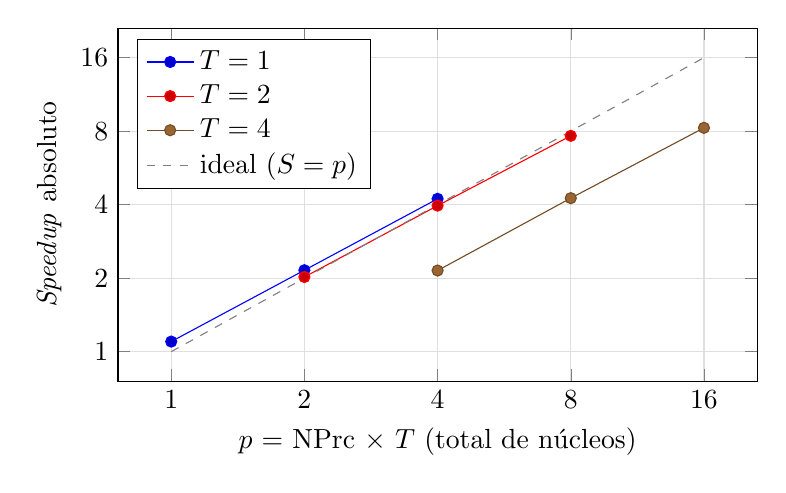
\begin{tikzpicture}
\begin{axis}[
    width=0.8\textwidth, height=0.5\textwidth,
    xmode=log, log basis x=2, ymode=log, log basis y=2,
    xlabel={$p$ = NPrc $\times$ $T$ (total de núcleos)}, ylabel={\emph{Speedup} absoluto},
    xtick={1,2,4,8,16}, xticklabels={1,2,4,8,16},
    ytick={1,2,4,8,16}, yticklabels={1,2,4,8,16},
    legend pos=north west, legend cell align=left, grid=major, grid style={gray!25},
]
\addplot+[mark=*] coordinates {(1,1.0998) (2,2.1554) (4,4.2261)};
\addlegendentry{$T=1$}
\addplot+[mark=*] coordinates {(2,2.0214) (4,3.9627) (8,7.6546)};
\addlegendentry{$T=2$}
\addplot+[mark=*] coordinates {(4,2.1490) (8,4.2524) (16,8.2523)};
\addlegendentry{$T=4$}
\addplot[dashed, gray, domain=1:16, samples=2] {x};
\addlegendentry{ideal ($S=p$)}
\end{axis}
\end{tikzpicture}
